\section{Witnessed choices on the grids}\label{sec:grid-behavior}\label{grid:section}

We now evaluate the sentence of Section~\ref{sec:sentence} on the
structures $A_b$ of Section~\ref{str:structures}.  Throughout this section,
$L\ge2$ and $b\in\F^{V_L}$; we identify the block graph with the underlying
box when this identification has been established.  The key point is that
every choice between two candidates is realized by a translation on at
most four faces followed by a scalar flow around one cycle.  These two
maps fix all previous choices, for every tree obtained from a parameter
$\alpha\in P$.

\subsection{Resolving parameters and face comparisons}

\begin{lemma}\label{grid:parameters}
Every structure $A_b$ passes the input check of Section~\ref{sec:sentence},
its block graph is the box on $V_L$, and its parameter set $P$ is nonempty.
\end{lemma}
\begin{proof}
The sort and block relations have the required interpretations.  Every
configuration in $X_v$ selects exactly one atom from $Y_e$ for each
$e\ni v$, and none from other edge blocks.  Each $X_v$ is nonempty by
Lemma~\ref{str:size}.  Thus the incidence test between blocks recovers
precisely the incidences of the box.  This graph is simple and connected,
and each edge has its two distinct endpoints, so all the input checks
hold.

Let $o=(0,0,0)$ and, for $i=1,2,3$, let $q_i$ be the corner whose $i$th
coordinate is $L-1$ and whose other coordinates are zero.  Distances in
the box are sums of absolute coordinate differences.  Indeed each step
changes one coordinate by one, giving the lower bound, and changing the
coordinates successively attains it within the box.  Hence, for
$v=(v_1,v_2,v_3)$,
\[
 d(o,v)-d(q_i,v)=2v_i-(L-1)\qquad(i=1,2,3).
\]
These are integer identities.  The four distances therefore determine
all three coordinates of $v$.  The tuple of blocks
$(X_o,X_{q_1},X_{q_2},X_{q_3})$ belongs to $P$.
\end{proof}

A face description in the sentence is an ordered description of a simple
four-cycle.  We use $\widehat f$ for such a description and $f$ for its
underlying elementary face; different descriptions may give the same
$f$.  For an atom $s\in Y_e$ and $f\in F(e)$, write $u_{s,f}\in\F^2$
for its coordinate belonging to that face.

\begin{lemma}[Recovering face coordinates]\label{grid:matching}
Every face description $\widehat f$ on $A_b$ describes an elementary face
$f$, and every elementary face has such a description.  For atoms $s,s'$
on any two sides of $f$, including the same side,
\begin{equation}\label{grid:match-equivalence}
 \operatorname{match}_{\widehat f}(s,s')
 \quad\Longleftrightarrow\quad u_{s,f}=u_{s',f}.
\end{equation}
Consequently, for $s=(e,u,z)$ and $s'=(e,u',z')$,
\begin{equation}\label{grid:base-equivalence}
 \operatorname{baseEq}_{Y_e}(s,s')\quad\Longleftrightarrow\quad u=u'.
\end{equation}
\end{lemma}
\begin{proof}
The four unit steps of a closed walk have zero sum in each coordinate.
They therefore consist either of two positive and two negative steps
in one direction, or of opposite pairs in two different directions.
The first possibility cannot give a simple cycle: at a greatest or least
coordinate reached, a reversal repeats the preceding vertex.  In the
second possibility no two successive steps can be opposites, since that
would also repeat a vertex.  The directions consequently alternate, and
the four vertices are exactly the corners of an elementary square.
Conversely, traversing any elementary square supplies a face description.

First consider adjacent sides $e,e'$ of $f$, meeting at $v$.  A
configuration containing $s\in Y_e$ and $s'\in Y_{e'}$ must satisfy
$u_{s,f}=u_{s',f}$ by the configuration equations.  Suppose this equality
holds.  The two sides share exactly the face $f$.  At $v$, choose one
vector for each face in $F(v)$, using the vector prescribed by $s$ or
$s'$ whenever that face meets the respective side; the only common
prescription is the assumed equality on $f$.  Assign the chosen vector
to both incident sides of each face.  This extends all vector coordinates
of the two given atoms without conflict.

Every vertex of the box has degree at least three, since $L\ge2$.
There is therefore an incident edge $h$ other than $e,e'$.  Keep the two
prescribed scalars, choose scalars arbitrarily on the remaining edges
other than $h$, and set
\[
 z_h=\epsilon_{vh}^{-1}
       \left(b_v-\sum_{g\ni v,\ g\ne h}\epsilon_{vg}z_g\right).
\]
The coefficient $\epsilon_{vh}$ is $1$ or $-1$, so it is invertible in
$\F$.  We have constructed a configuration in $X_v$ incident with both
given atoms.  This proves Equation~\eqref{grid:match-equivalence} for
adjacent sides, for every charge and including boundary vertices.

For opposite sides, the definition uses an atom on a side adjacent to
both; for two atoms on the same side, it uses an atom on the next side
in the description.  The adjacent-side case shows that the two required
tests hold precisely when this intervening atom has the same $f$-vector
as both $s$ and $s'$.  Every vector in $\F^2$ occurs on the intervening
side.  The two configuration witnesses are independent, even when their
vertex blocks coincide.  Thus such an intervening atom exists exactly
when $u_{s,f}=u_{s',f}$.  Finally, the descriptions containing $e$ cover
exactly its incident faces, which proves
Equation~\eqref{grid:base-equivalence}.
\end{proof}

\subsection{Transporting candidates while fixing the history}

Fix any $\alpha\in P$, and let $T=T(\alpha)$ be its spanning tree.
List the edges outside $T$ in the order defined from $\alpha$ as
$e_1,\ldots,e_r$.  Say that $x$ is a compatible prefix of length $j$
if it consists of one atom on each of $e_1,\ldots,e_j$ and no other
elements, and if its atoms have equal $f$-vectors whenever their edges
belong to a common face $f$.  The empty set is the compatible prefix of
length zero.

For $j<r$ and a compatible prefix $x$ of length $j$, put $e=e_{j+1}$
and
\[
 F_x(e)=\{f\in F(e):\text{some edge of }f\text{ has a selected atom in }x\}.
\]
For each $f\in F_x(e)$, compatibility gives a well-defined common vector
$v_f$.  Lemma~\ref{grid:matching} identifies the candidate set exactly:
\begin{equation}\label{grid:candidates}
 D(\alpha,x)=\{(e,u,z)\in Y_e:
                    u_f=v_f\text{ for all }f\in F_x(e)\}.
\end{equation}
This set is nonempty: its remaining vector coordinates and its scalar
$z$ are unrestricted.  We next prove that the witness guard succeeds on
this entire set.

\begin{proposition}[Transitivity for every parameter tree]
\label{grid:transitivity}
Let $A_b$ be a grid structure, $\alpha\in P$, and $x$ a compatible prefix
of length $j<r$.  For every ordered pair $s,s'\in D(\alpha,x)$ there is
$g\in M(\alpha,x)$ with $g(s)=s'$.  The map $g$ preserves the full input,
fixes every block setwise, and fixes every atom of $x$ individually.
Consequently every selection path for $\alpha$ chooses one atom from
each edge outside $T$, in order, maintains compatibility, and then
stabilizes with the dummy choice.  All its witnessing maps respect
$\alpha$ and the entire preceding history.
\end{proposition}
\begin{proof}
Write $s=(e,u,z)$ and $s'=(e,u',z')$.  We construct a map from the local
pool $\mathcal L$ and then one from the cycle pool
$\mathcal C(\alpha,x)$, in the order used to define $M$.
Figure~\ref{grid:figure} illustrates the two transformations.

Define $a\in C_F$ by
\[
 a_f=\begin{cases}
       u'_f-u_f,&f\in F(e),\\
       0,&f\notin F(e).
     \end{cases}
\]
Let $\ell=h_{a,0}$ be the automorphism from
Proposition~\ref{str:action}.  A nonzero $a_f$ can occur on at most four
faces.  Outside the edge and vertex blocks belonging to these faces,
$\ell$ is the identity by Equation~\eqref{str:edge-action} and the
induced action on configurations.  Each face has four sides and four
vertices, so $\ell$ moves atoms in at most sixteen edge blocks and
sixteen vertex blocks.  The block bounds in Lemma~\ref{str:size} give
\[
 |\{t\in A_b:\ell(t)\ne t\}|
 \le16(3^9+3^{29})=B.
\]
Thus $\ell$ occurs in the local pool: if its support is nonempty, list
the moved atoms and their images in the two indexing tuples and pad
them with repetitions; if its support is empty, use the explicitly
included identity.  This represents the whole permutation because it
is the identity outside the listed atoms.

For $f\in F_x(e)$, Equation~\eqref{grid:candidates} gives $a_f=0$.
Every face with a nonzero translation therefore contains no previously
selected edge.  All face coordinates and the scalar of each atom in
$x$ are unchanged, so $\ell$ fixes $x$ pointwise.  On the current
candidate, its value is
\begin{equation}\label{grid:post-local-scalar}
 \ell(s)=(e,u',\widetilde z),\qquad
 \widetilde z=z+\frac12\sum_{f\in F(e)}c^f_e\omega(a_f,u_f).
\end{equation}
It remains to correct $z'-\widetilde z$, which is the scalar discrepancy
after this translation.

If $z'=\widetilde z$, take the identity from the cycle pool.  Otherwise
put $\eta=z'-\widetilde z\in\{1,-1\}\subseteq\F$.  The cycle pool
enumerates every auxiliary vertex block $o$, so it includes the block
at the coordinate origin.  For this choice of $o$, the function
$d(o,v)=v_1+v_2+v_3$ increases by one along every positive coordinate
edge.  Its labels $1$ and $2=-1$ consequently agree with signed edge
traversal in the fixed coordinate orientations, regardless of the root
or shape of $T$.

Choose the ordering $(U,V)$ of the endpoints of $e$ so that traversing
$e$ from $U$ to $V$ has sign $\eta$.  Follow this edge and then the
unique tree path from $V$ to $U$.  Because $e\notin T$, this is a simple
cycle.  Let $k\in\F^{E_L}$ have coefficient $1$ or $-1$ on each edge
according to the traversal orientation and coefficient zero elsewhere.
At each vertex one traversed edge enters and one leaves, so
\begin{equation}\label{grid:cycle-circulation}
 \partial k=0,\qquad k_e=\eta,\qquad
 \operatorname{supp}(k)\subseteq T\cup\{e\}.
\end{equation}

For the indices just chosen, the cycle-pool relation is exactly the
graph of $h_{0,k}$.  To check this assertion on an edge of the cycle,
Lemma~\ref{grid:matching} makes its $\operatorname{baseEq}$ condition
equivalent to equality of all vector coordinates.  For equal vectors,
alternation gives $\omega(u_f,u_f)=0$, so the
$\Zrel_{\delta}$ condition becomes $z'-z=\delta=k_h$.  It therefore
pairs each edge atom with precisely its scalar translate by $k_h$.
Off the cycle the relation is the identity, as is $h_{0,k}$.  On a
vertex block, its definition pairs a configuration with precisely the
tuple of these translated incident states.  That tuple is a
configuration by Proposition~\ref{str:action}, and there is exactly
one configuration atom for each permitted tuple.  This proves the
assertion on the configuration sort as well.

Call this cycle map $c$.  By Equation~\eqref{grid:cycle-circulation},
it fixes every earlier selected atom: all their edges are outside $T$
and different from $e$.  Both $c$ and $\ell$ preserve every block and
the full vocabulary, so the composition $g=c\circ\ell$ passes the
filter defining $M(\alpha,x)$.  Equations~\eqref{grid:post-local-scalar}
and~\eqref{grid:cycle-circulation} give $g(s)=s'$.  The same conclusion
holds in the zero-discrepancy case with $c$ equal to the identity.

We have proved nonemptiness and the witness guard for every compatible
prefix with an unprocessed edge.  The next real choice extends that
prefix by one atom and preserves compatibility by
Equation~\eqref{grid:candidates}.  Induction starts at $x=\emptyset$.
After all $r$ edges have been processed, there is no next edge; the
dummy choice leaves the state unchanged and is witnessed by the
identity.  Finally, fixing each block fixes the tuple $\alpha$, and
fixing all atoms of the current prefix fixes each earlier prefix as
a set.  Thus the maps satisfy the parameter and history requirements
of witnessed symmetric choice.
\end{proof}

\begin{figure}[tb]
 \centering
 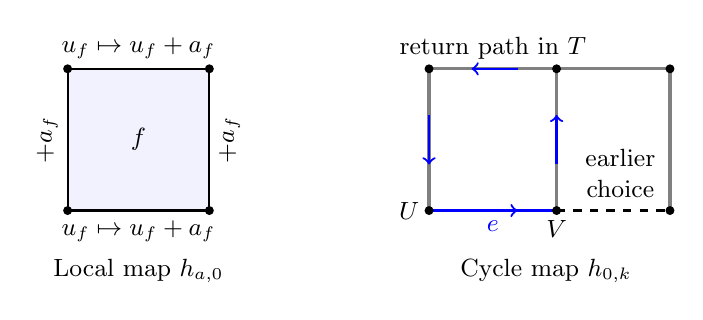
\begin{tikzpicture}[scale=.9, every node/.style={font=\small}]
  \begin{scope}
    \fill[blue!5] (0,0) rectangle (2,2);
    \draw[thick] (0,0)--(2,0)--(2,2)--(0,2)--cycle;
    \foreach \x/\y in {0/0,2/0,2/2,0/2}
      \fill (\x,\y) circle (1.8pt);
    \node at (1,1) {$f$};
    \node[below] at (1,0) {$u_f\mapsto u_f+a_f$};
    \node[above] at (1,2) {$u_f\mapsto u_f+a_f$};
    \node[rotate=90,above] at (0,1) {$+a_f$};
    \node[rotate=90,below] at (2,1) {$+a_f$};
    \node at (1,-.85) {Local map $h_{a,0}$};
  \end{scope}
  \begin{scope}[xshift=5.1cm]
    \coordinate (u) at (0,0);
    \coordinate (v) at (1.8,0);
    \coordinate (a) at (0,2);
    \coordinate (b) at (1.8,2);
    \coordinate (c) at (3.4,2);
    \coordinate (d) at (3.4,0);
    \draw[very thick,gray] (u)--(a)--(b)--(v);
    \draw[very thick,gray] (b)--(c)--(d);
    \draw[thick,blue] (u)--(v);
    \draw[thick,dashed] (v)--(d);
    \draw[->,blue,thick] (.6,0)--(1.25,0);
    \draw[->,blue,thick] (1.8,.65)--(1.8,1.35);
    \draw[->,blue,thick] (1.25,2)--(.6,2);
    \draw[->,blue,thick] (0,1.35)--(0,.65);
    \foreach \p in {u,v,a,b,c,d}
      \fill (\p) circle (1.8pt);
    \node[left] at (u) {$U$};
    \node[below] at (v) {$V$};
    \node[below,blue] at (.9,0) {$e$};
    \node[above] at (.9,2) {return path in $T$};
    \node[above,align=center] at (2.7,.05) {earlier\\choice};
    \node at (1.65,-.85) {Cycle map $h_{0,k}$};
  \end{scope}
\end{tikzpicture}

 \caption{The two parts of a candidate transport.  Left: a translation
 on one face adds the same vector $a_f$ to its four sides and acts on
 their endpoint configurations; the construction uses at most four
 such faces.  The left panel shows only vector coordinates; the scalar
 correction for $h_{a,0}$ is given in
 Equation~\eqref{grid:post-local-scalar}.  Right: the new edge $e$ (blue)
 and its return path in $T$ carry a circulation.  Other tree edges are grey; a previously
 selected edge outside $T$ is dashed and is untouched by the
 circulation.  The picture shows only the relevant part of the tree.}
 \label{grid:figure}
\end{figure}

\subsection{Extending a terminal selection}

Proposition~\ref{grid:transitivity} shows that the output test always
receives a complete, compatible assignment outside its tree.  To
evaluate that test, we must determine whether the remaining edge
states can satisfy all vertex equations.  The vector coordinates
extend face by face; the scalar equations reduce to divergence on a
tree.

\begin{lemma}[Solving divergence on a tree]\label{grid:tree-divergence}
Let $T$ be a finite tree on vertex set $V$, orient its edges arbitrarily,
and write $\partial_T$ for its signed incidence map.  Let $r\in\F^V$
satisfy $\sum_{v\in V}r_v=0$.  There is a unique
$z\in\F^{E(T)}$ with $\partial_T z=r$.
\end{lemma}
\begin{proof}
For a one-vertex tree, the sum condition says $r=0$, and the empty edge
assignment is the unique solution.  Otherwise let $v$ be a leaf, $h$
its incident edge, and $w$ its neighbor.  The equation at $v$ forces
$z_h=\epsilon_{vh}^{-1}r_v$.  Delete $v$ and $h$; keep all other
required divergences except that at $w$, where set
\[
 r'_w=r_w-\epsilon_{wh}z_h=r_w+r_v.
\]
The new required divergences still sum to zero.  Induction supplies
the unique solution on the smaller tree, which together with the
forced value on $h$ solves all the original equations.  Each deleted
edge was forced, proving uniqueness as well.
\end{proof}

\begin{theorem}[Opposite grid answers]\label{grid:separation}
For every $L\ge2$, the fixed sentence $\Phi$ of
Section~\ref{sec:sentence} evaluates to true on $A_{b^0}$ and to false
on $A_{b^1}$.  For either structure, every parameter $\alpha\in P$
and every terminal selection gives the stated output value, and no
evaluation produces $\dagger$.
\end{theorem}
\begin{proof}
By Lemma~\ref{grid:parameters}, both inputs pass the check and have a
nonempty parameter set.  Fix any $\alpha\in P$ and any terminal
selection $x$.  Proposition~\ref{grid:transitivity} says that $x$ is a
complete compatible assignment on the edges outside $T=T(\alpha)$.

First work in $A_{b^0}$.  For each elementary face $f$, choose its
vector $v_f\in\F^2$ to be the one already prescribed by $x$ if an
edge of $f$ was selected, and choose any vector otherwise.
Compatibility makes each prescription unambiguous.  Give every edge
$e$ the vectors $(v_f)_{f\in F(e)}$.  This preserves all selected
vector coordinates and satisfies all face agreements at vertices.

Keep the selected scalars $z_e$ on $e\notin T$, and define the
divergence still required from tree edges by
\[
 r_v=b^0_v-\sum_{e\notin T}\epsilon_{ve}z_e.
\]
Every edge contributes once with each sign, and $\sum_v b^0_v=0$;
therefore $\sum_v r_v=0$.  Lemma~\ref{grid:tree-divergence} supplies
the scalars on $T$.  The resulting full edge assignment has divergence
$b^0$ and satisfies every face agreement.  Its incident tuple at each
vertex is consequently a configuration atom, and neighboring tuples
specify the same edge atom.  By Lemma~\ref{sen:tree-test}, the output
test accepts $x$.

Now work in $A_{b^1}$.  If the output test accepted $x$,
Lemma~\ref{sen:tree-test} would supply configurations agreeing on a
single atom on every edge.  Let $z_e$ denote the scalar of that common
atom.  The equations at all vertices would give
\[
 1=\sum_{v\in V_L}b^1_v
   =\sum_{v\in V_L}\sum_{e\in E_L}\epsilon_{ve}z_e
   =\sum_{e\in E_L}(1-1)z_e=0
 \quad\text{in }\F,
\]
a contradiction.  Thus every terminal selection is rejected.

The witness and resource conclusions of
Proposition~\ref{sen:all-input} apply to these calls, so their values are
Boolean.  The output value just proved is the same for every terminal
selection for each parameter.  Since $P$ is nonempty, the outer
existential aggregation defining $\Phi$ is true on $A_{b^0}$ and false
on $A_{b^1}$, as asserted.
\end{proof}
